\section{Background}
A new exciting segment of the technology sector has sprung up recently – indoor navigation with a catalyst of growth in indoor navigational research. Current solutions on the market cater very well for basic navigation of large open public spaces, though failing to display competencies to more complex navigational requirements coupled with even proportions of navigational, and interactive content with well-presented data. Through the use of AR, this concept can provide an interactive solution for museums.

Since most museums use portable audio guides, user experiences can be vastly improved by the use of a smartphone. Currently only a few solutions can be found; the Orpheo group provide a unique app for each individual museum though their solution is somewhat cumbersome to regular museum users who wish to have a hassle-free setup. The appeal to museums and by virtue of this, museum-goers having one app whereby the user can simply walk into a museum or exhibition, and be greeted with relevant information would be a key differentiating factor \cite{microsoft}. Even though the intention is to create one app for every museum and exhibition for the project, each client would have a large input on the content of their institution within the app. 

If a museum wanted a solution for navigation, due to the low number of museum-specific competitors, would choose standard indoor mapping softwares \cite{murphy}. While there are many options out there from Google, and Mapspeople \cite{mapspeople} who provide this, they lack important exigences that are imperative for museums like heavily integrated augmented reality, and intelligent tour guiding from your location.

\section{AR Libraries}
The group evaluated three libraries before developing any software. ARKit developed by Apple for its native iOS platform, the ARCore library by Google for Android systems, and Vuforia - a cross-platform SDK built by PTC for Unity/Android, specialising in image recognition.

\subsection{ARKit}
ARKit was a strong candidate in becoming the library of choice because of its nativity to iOS devices. The prototype built would hover over an image, in this scenario - the Mona Lisa, and the device would recognise the painting. Subsequently, it would display information about it, and if scanned again, a green tick would be displayed on the screen.

Although the application is only written in Swift, it has more thorough, and straight-forward documentation than Android's ARCore and PTC's Vulforia. This would make the idea easier to manifest because the debugging process would likely run more smoothly. However, due to the lack of the group's familiarity with the platform, only one person was able to partake in creating the image recognition prototype (Figure~\ref{fig:arlibrary1}), making it an unfit library to move forward with.

\begin{figure}[H]
	\centering  
	\begin{tabular}{cc}
	  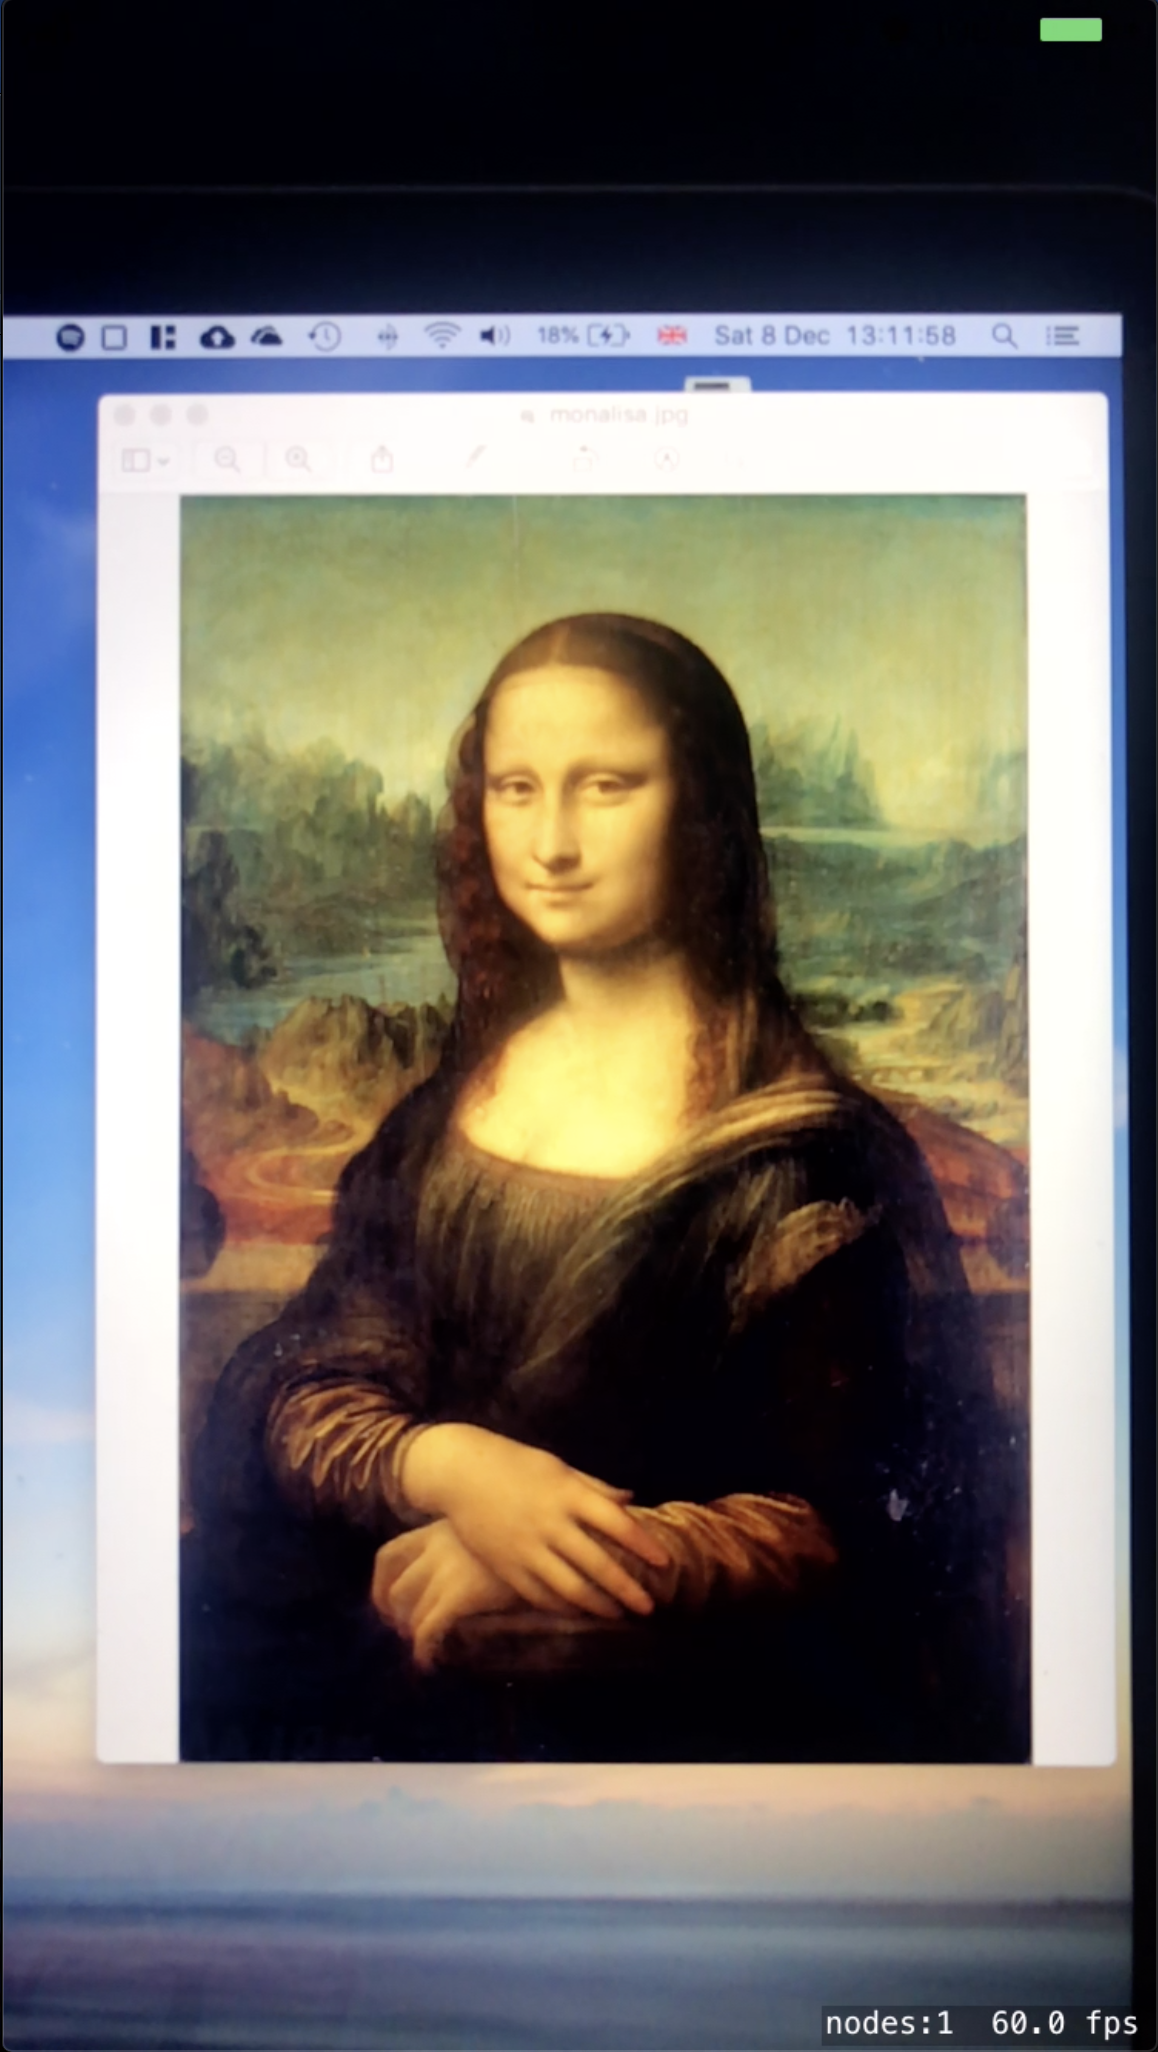
\includegraphics[width=60mm, height=100mm]{prototypes/ar/ios/1.png} &   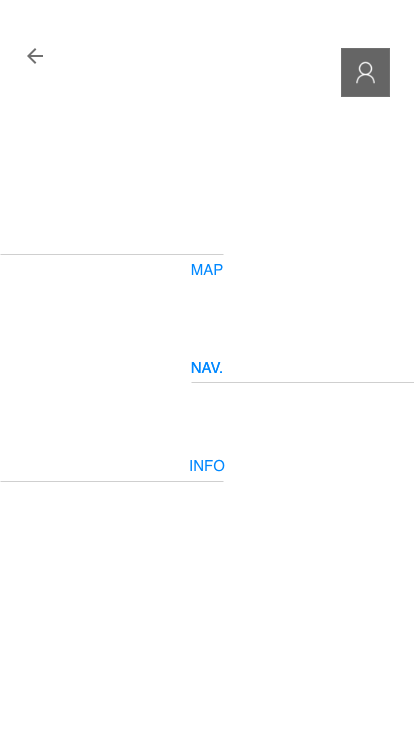
\includegraphics[width=60mm, height=100mm]{prototypes/ar/ios/2.png} \\
	(a) Camera over image & (b) Image recognised and displaying information \\[6pt]
	\multicolumn{2}{c}{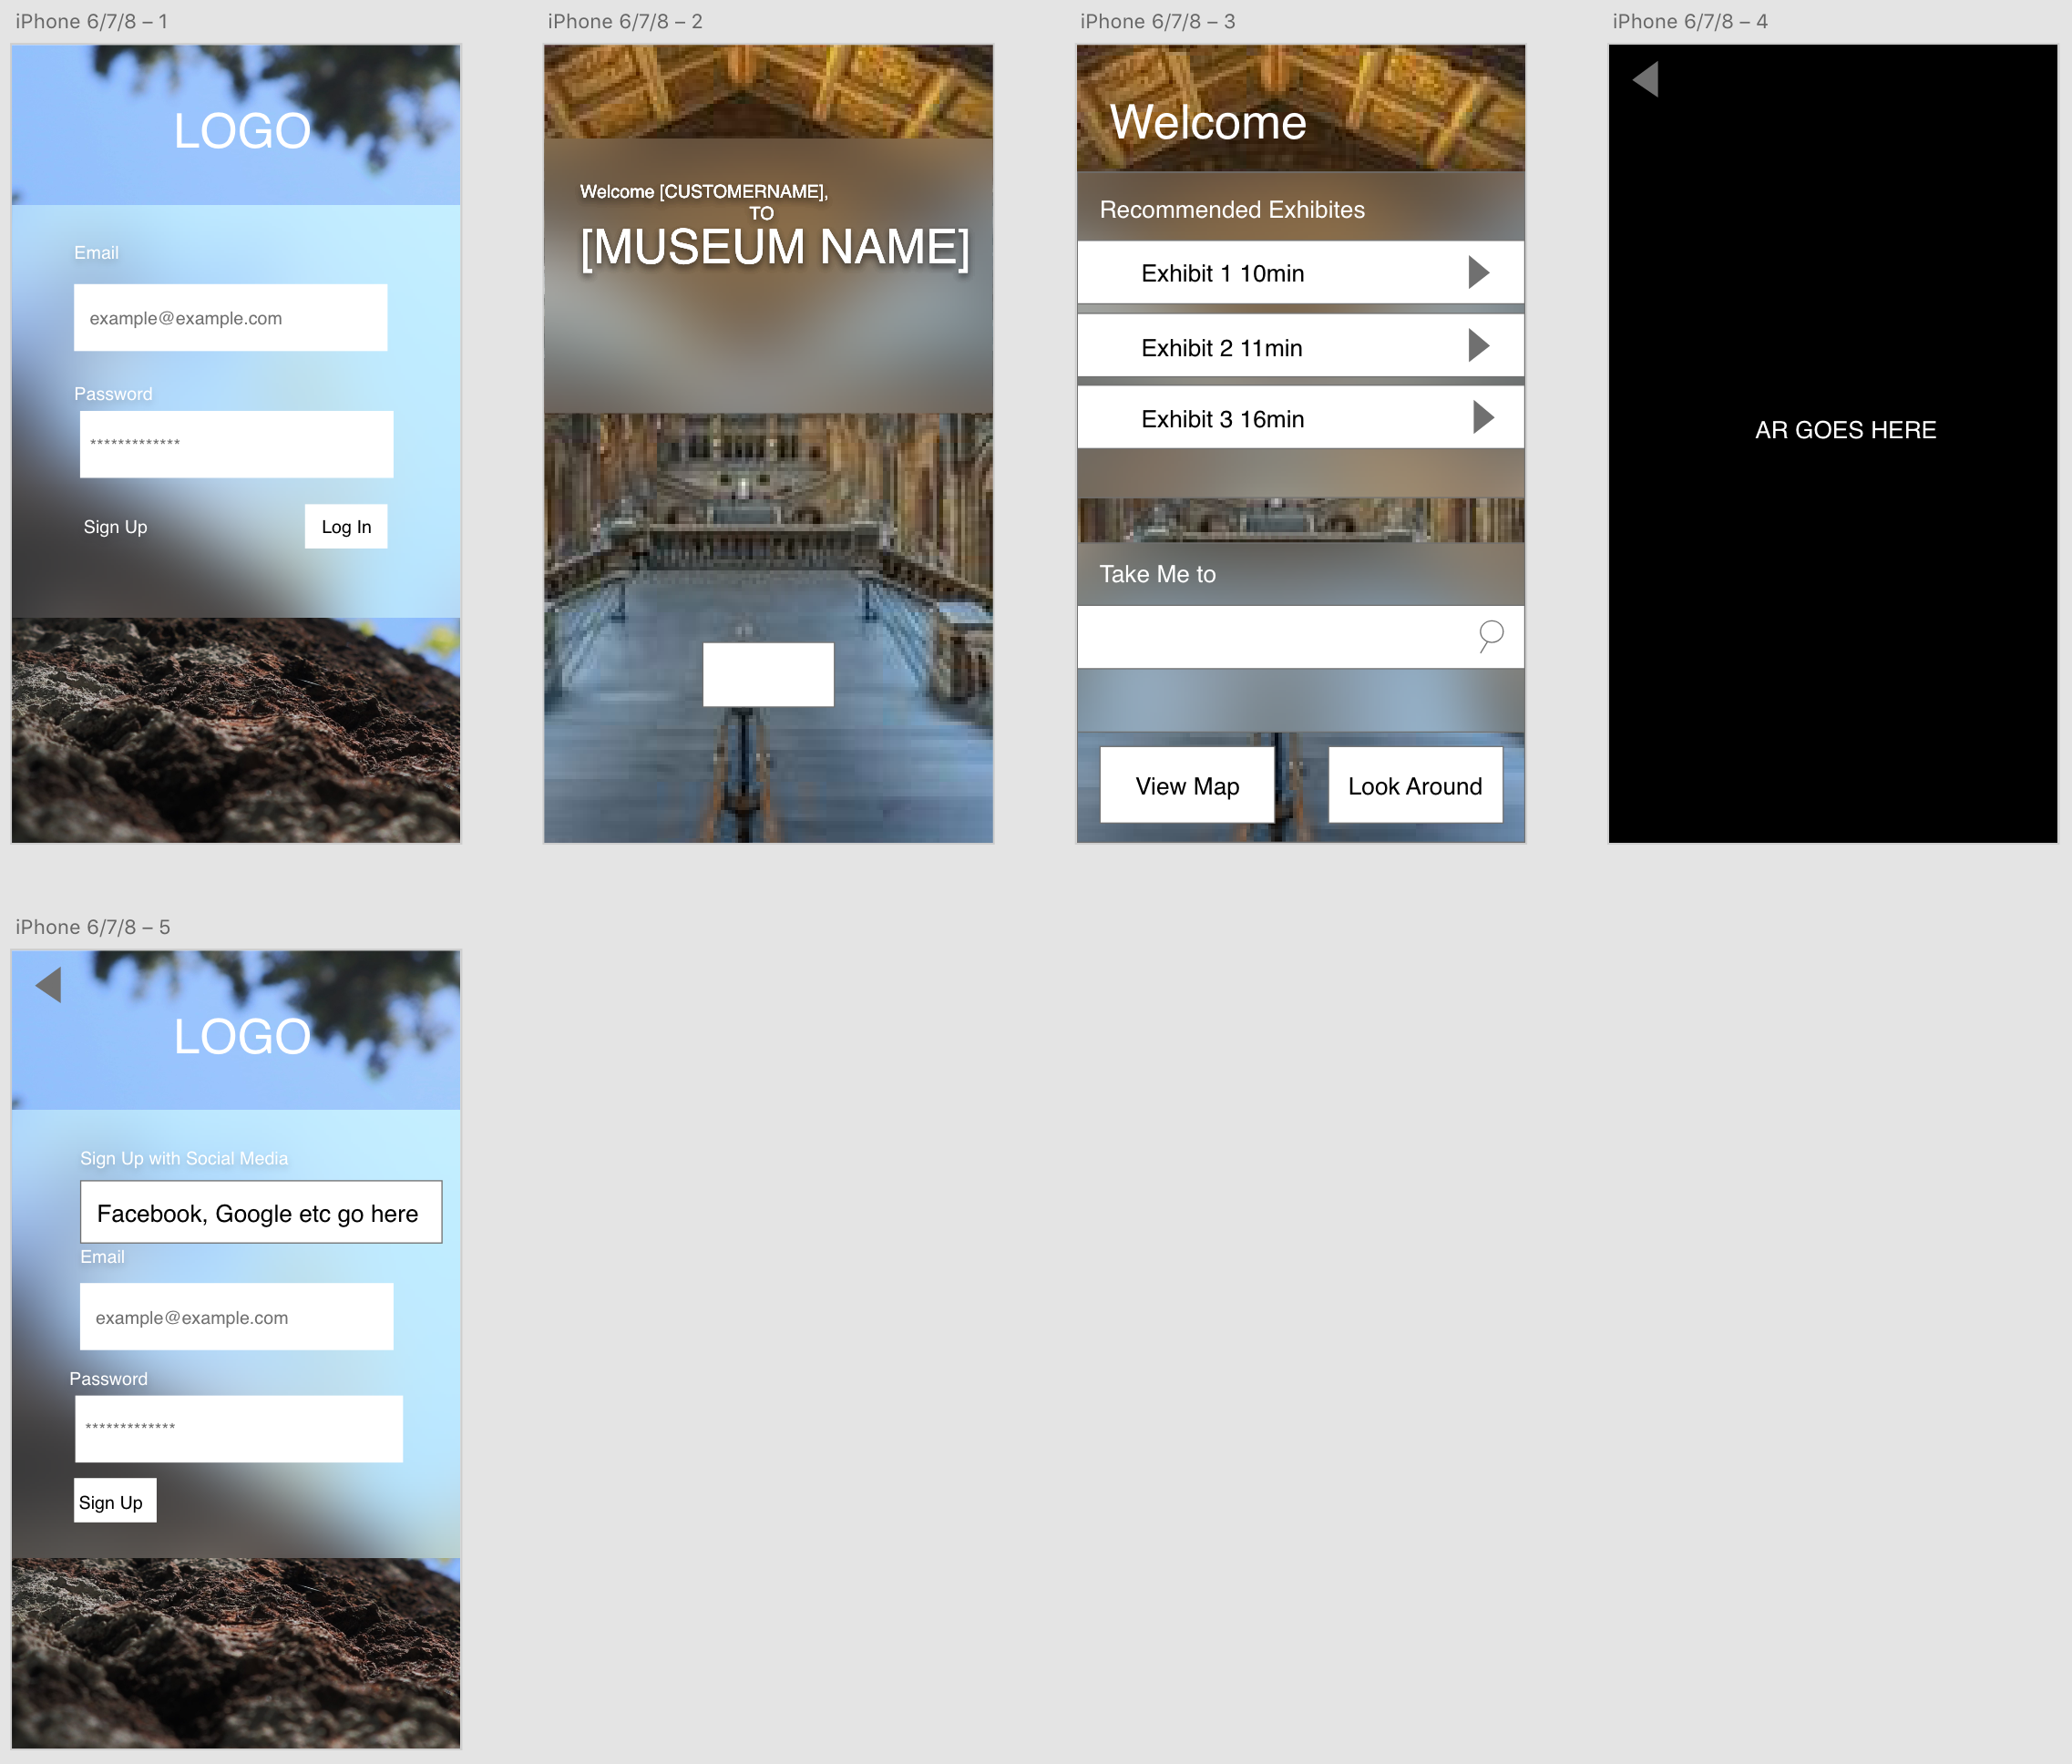
\includegraphics[width=60mm, height=100mm]{prototypes/ar/ios/3.png} }\\
	\multicolumn{2}{c}{(c) Image scanned before; showing the green tick}
	\end{tabular}
	\caption{ARKit prototyping on iOS device}
	\label{fig:arlibrary1}
\end{figure}

\subsection{Vuforia}
Unity is a cross-platform game engine, used to test a simple AR camera prototype where the device’s camera hovers over an image, and displays information about that image on the device. The application was built using Vuforia, an SDK that enables recognition, and tracking of image targets. This library can be used for the exploration case in the use case model. Although, there are a lack of tools for locating user's current location compared to Android.

The Vuforia library was used to test a simple AR camera prototype where the device’s camera hovers an image, and displays information about that image on the device.

\begin{figure}[H]
	\centering  
	\begin{tabular}{cc}
	  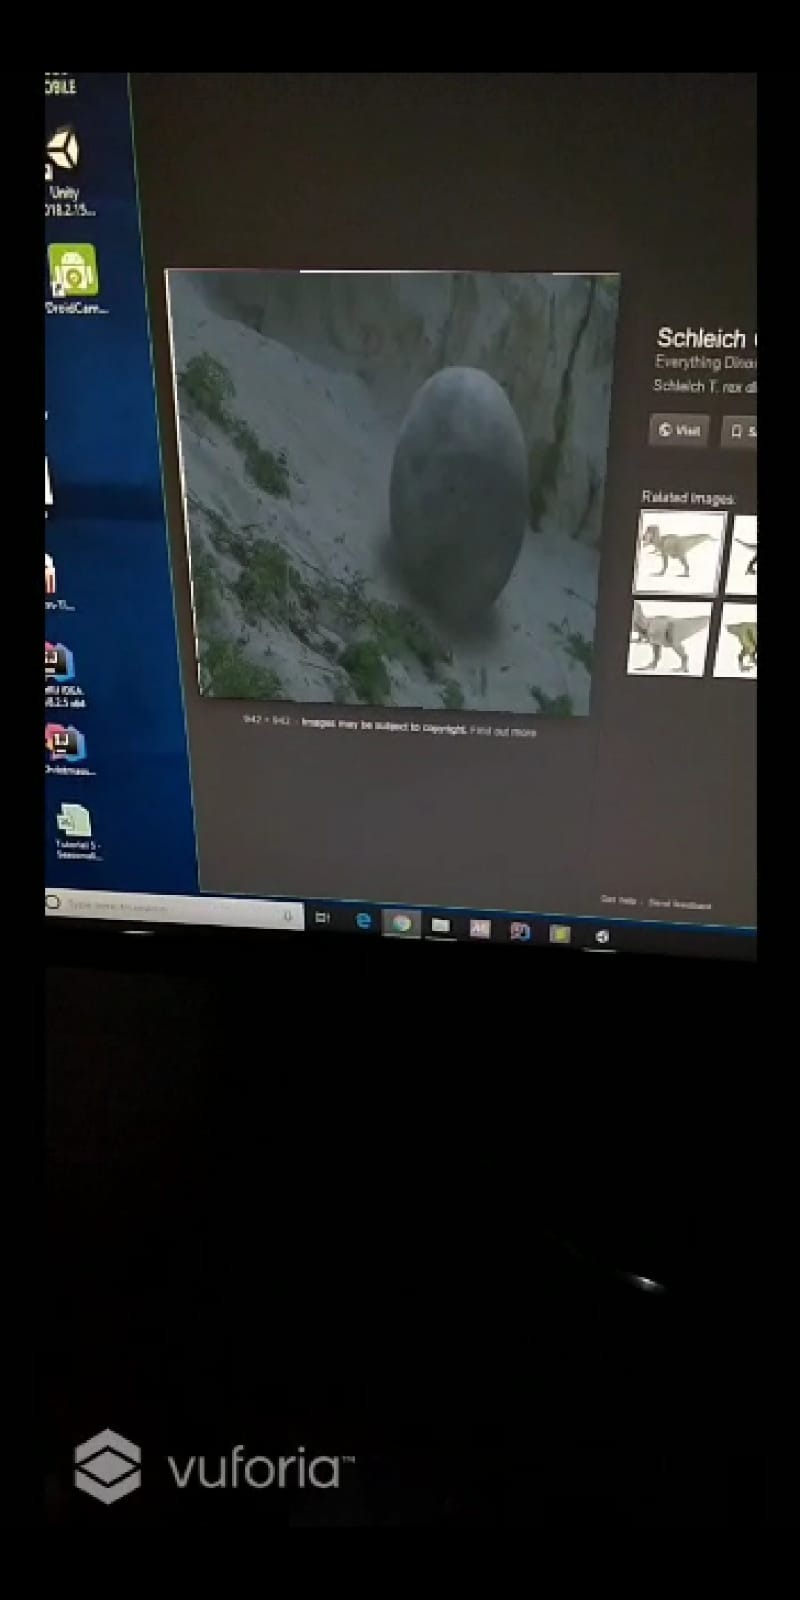
\includegraphics[width=60mm, height=100mm]{prototypes/ar/vulforia/1.jpeg} &   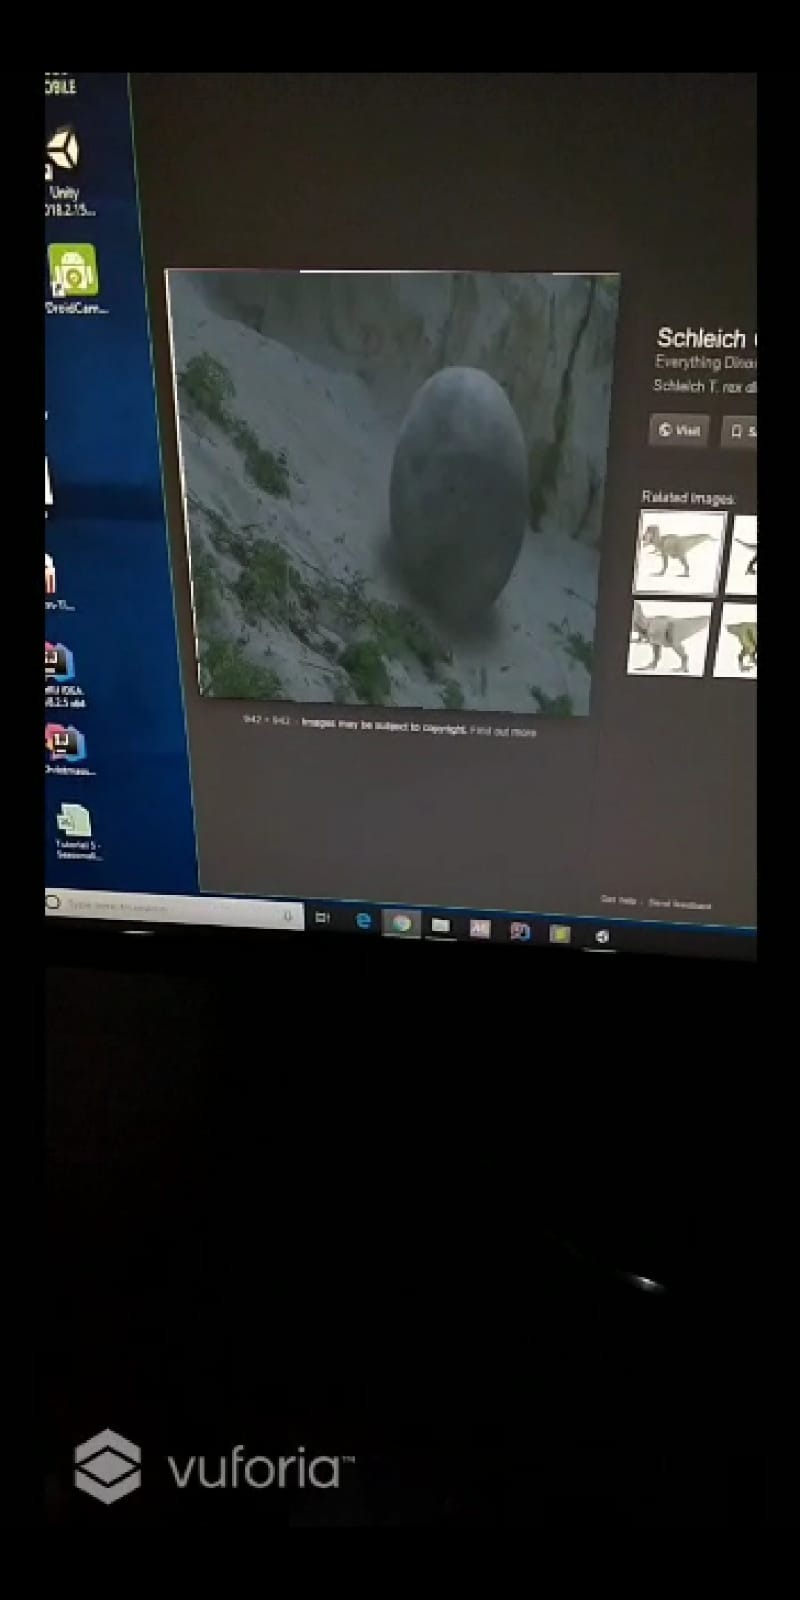
\includegraphics[width=60mm, height=100mm]{prototypes/ar/vulforia/2.jpeg} \\
	(a) Camera over image & (b) Video superimposed on top of image\\[6pt]
	\end{tabular}
	\caption{Vuforia prototyping on Android device}
	\label{fig:arlibrary2}
\end{figure}

\subsection{ARCore}
ARCore was used to create an AR experience (Figure~\ref{fig:arlibrary3}) giving the user the ability to superimpose a 3D object when the camera is focused on a flat surface. This prototype simply recognised a flat surface, and when detected the user could place the Android robot on the surface.

During the process it was found that unlike ARKit, the library is suitable with Java/Kotlin, hence the group would have an easier time acclimating the nature of ARCore. As ARCore is a native Android SDK, it can be integrated with other Android features such as Android's GPS, and Android's WiFi libraries. Despite this, the documentation was scattered and vague, making it difficult to debug with. After exploring this prototyping process, and discussing the accessibility of ARCore, and Android to the stakeholders, the group distinguished it as the most suitable library for the project.

\begin{figure}[H]
	\centering  
	\begin{tabular}{cc}
	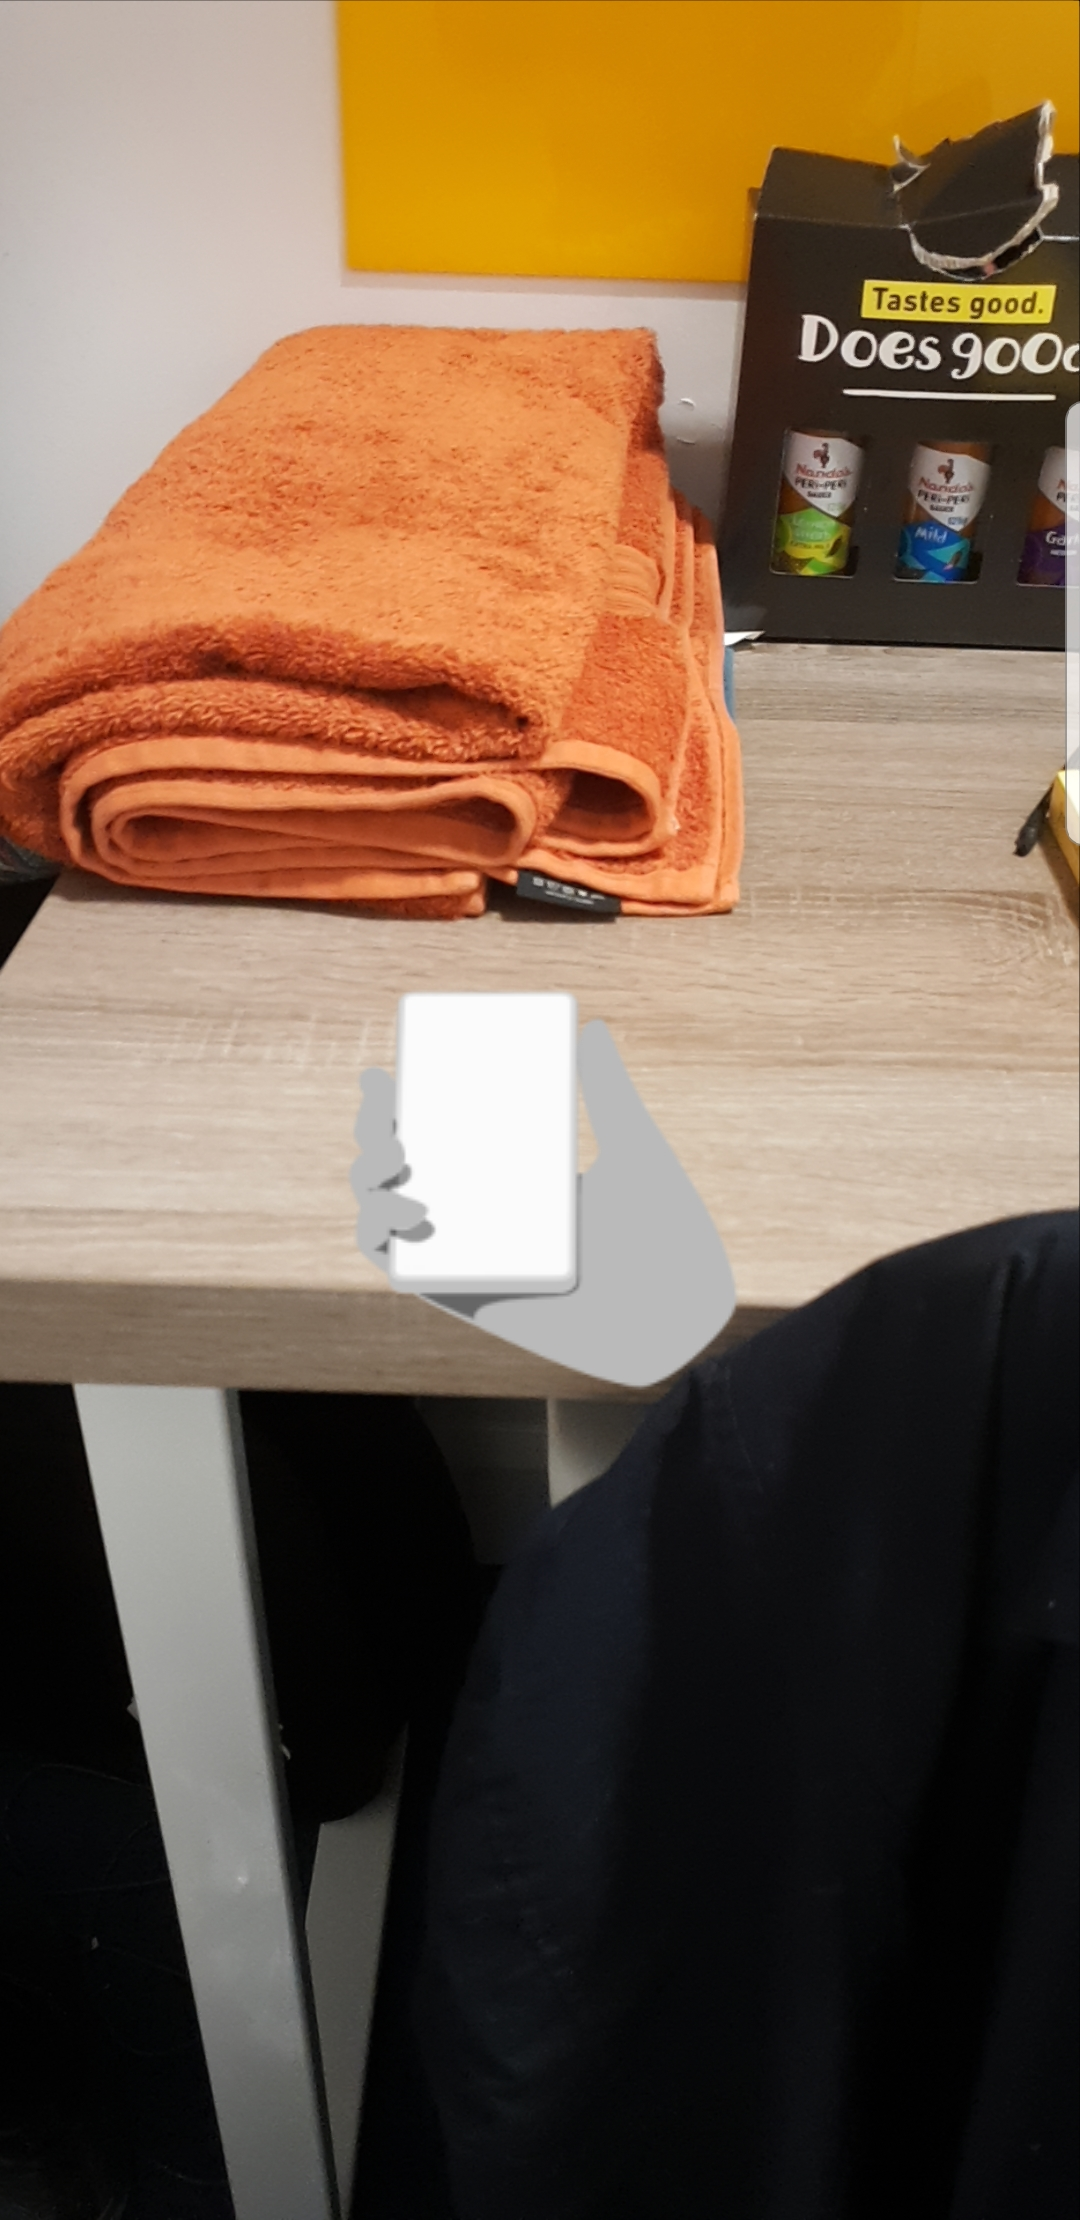
\includegraphics[width=60mm, height=100mm]{prototypes/ar/android/1.jpg} & 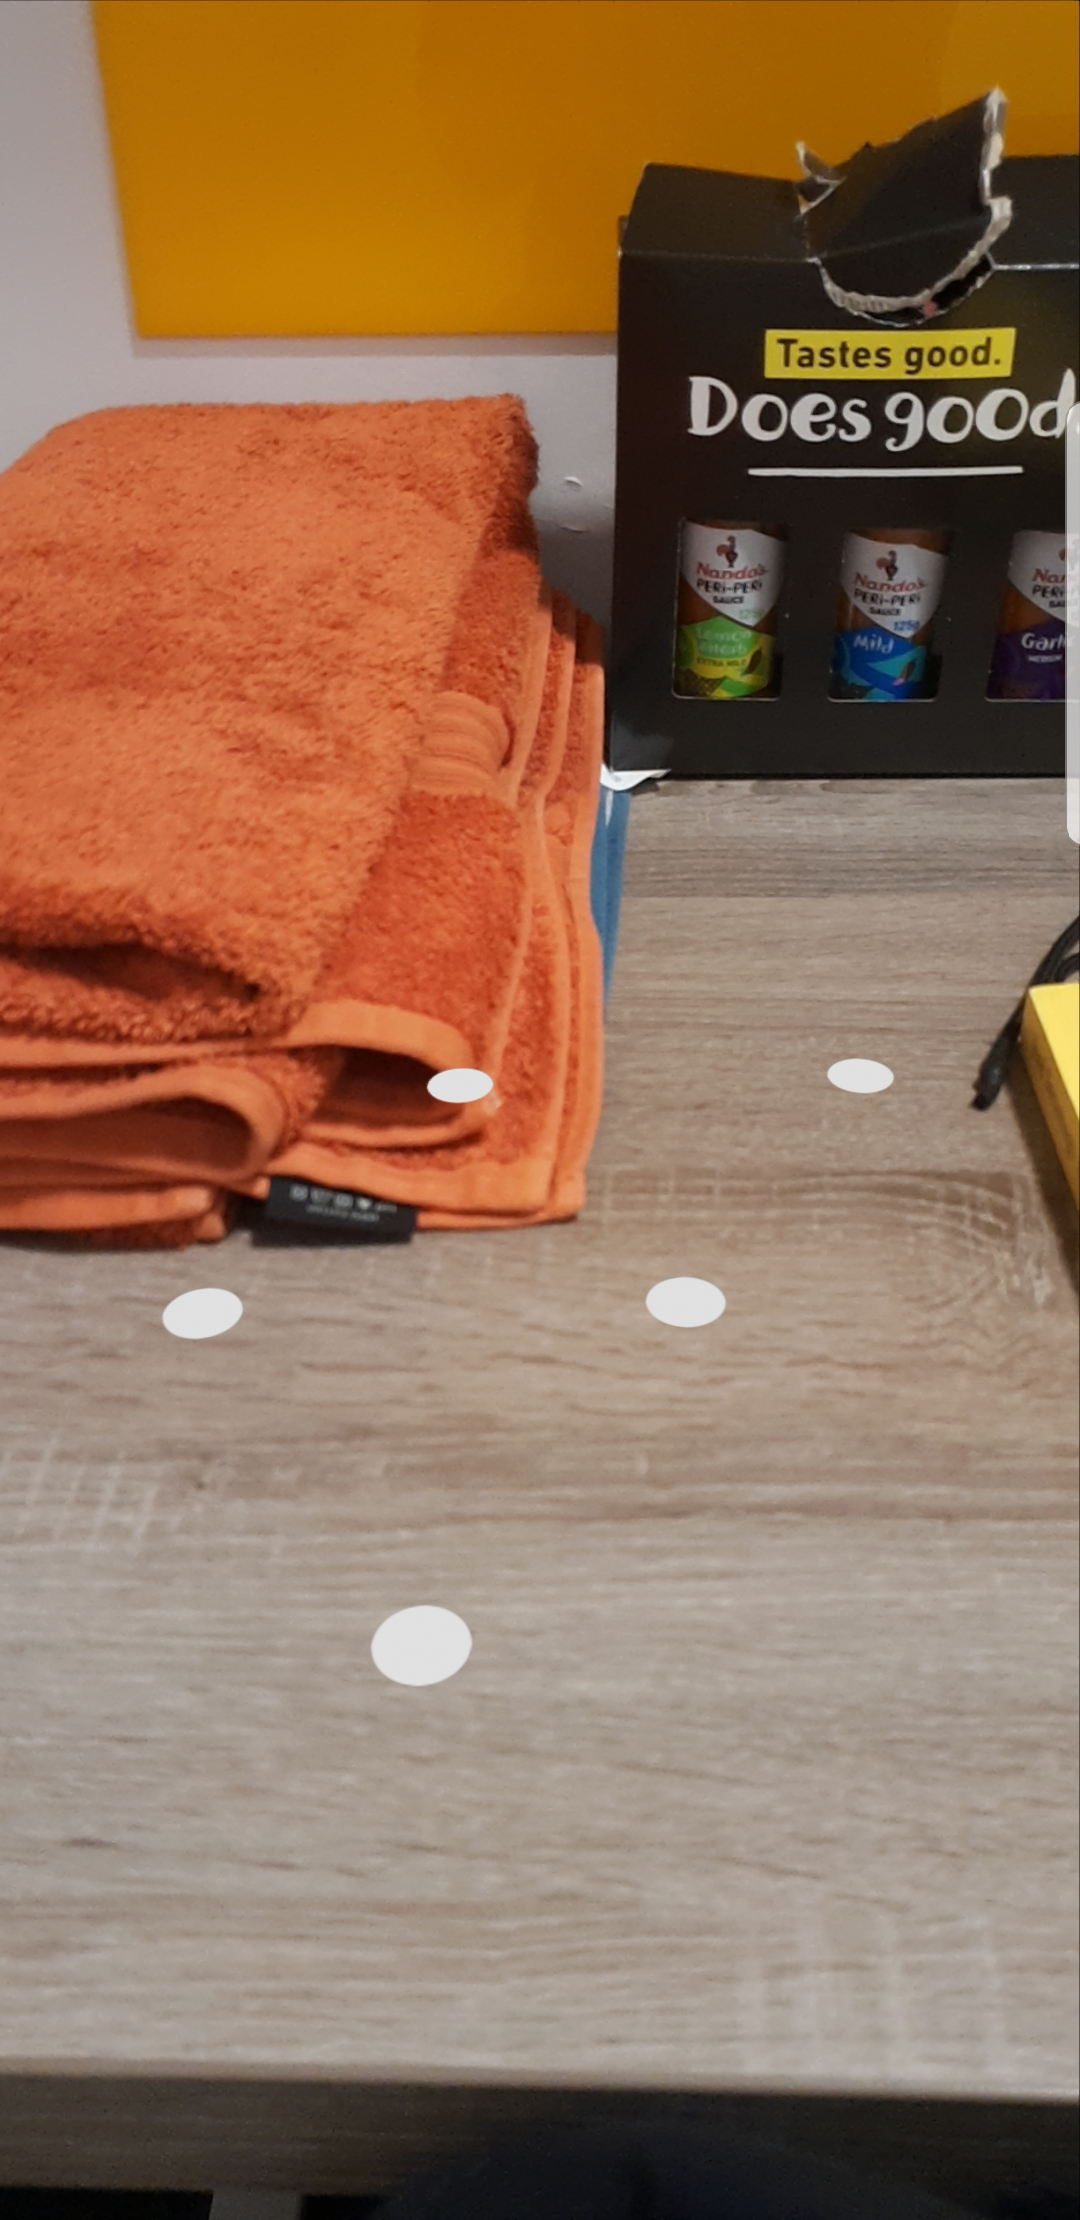
\includegraphics[width=60mm, height=100mm]{prototypes/ar/android/2.jpg} \\
	(a) Initial view & (b) Detection of surface \\[6pt]
	\multicolumn{2}{c}{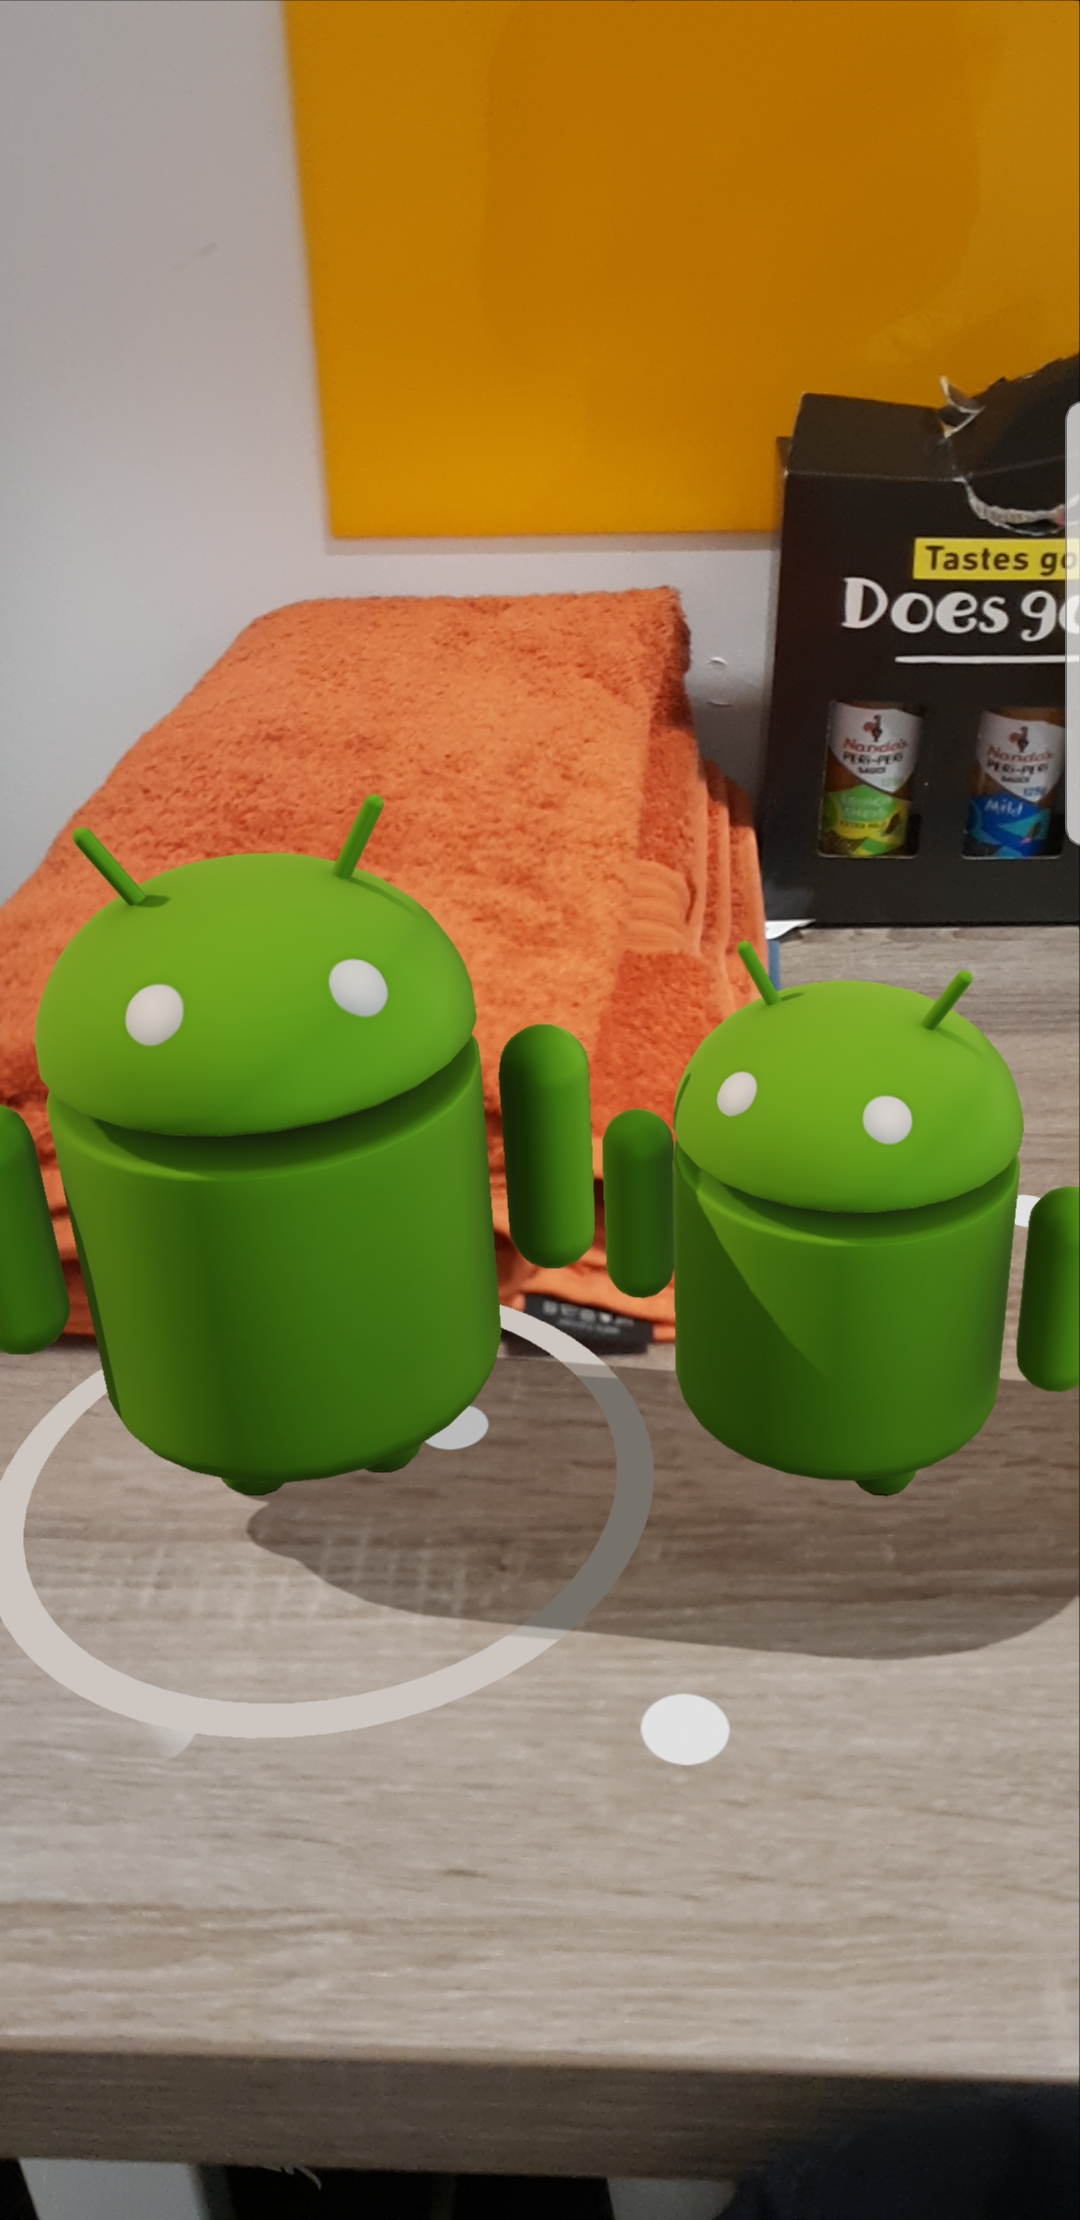
\includegraphics[width=60mm, height=100mm]{prototypes/ar/android/3.jpg} }\\
	\multicolumn{2}{c}{(c) Objects superimposed on surface}
	\end{tabular}
	\caption{ARCore prototyping on Android device}
	\label{fig:arlibrary3}
\end{figure}

\section{Software Architecture}
To aid with selecting AR technologies, two operating systems were analysed to identify the potential risks, and verify the quality of software prototypes in design.

\subsection{Android}
An open-source OS developed by Google, it provides an SDK for development. It uses the \textit{.apk} extension that can be downloaded, and installed on mobile phones. The Android emulator is nearly three time faster in CPU speed compared to Apple, allowing for smoother development of non-camera features. GPS location data is easier to use in Android due to how packages are imported into files, so there is low coupling. Further, the creation of user interface elements is straightforward, and can be executed on a wide variety of devices. However, it is harder creating more complex layouts and animations, and there is a steeper learning curve in Android development compared to other operating systems.

\subsection{iOS}
iOS is a mobile operating system developed by Apple, providing the ARKit SDK for development of the application. Only Swift is compatible with iOS, though this is notoriously an easy language to learn, and develop apps on. Apple devices have more accurate accelerometers, and gyroscope, enabling stable and fast motion tracking \cite{pmc}. There are also fewer dependencies compared to Android, hence application load time is faster. Yet, there are limitations of the ARKit map, and the application would only support fewer devices.

\section{Hardware}
As part of the exploration it was recommended, based off lengthy research, and the project’s domain expert's advice the need for a physical beacon. 

This role of this beacon was to broadcast a signal; three main current technologies exist exist: optical infra-red, Bluetooth and, WiFi. Speaking to the project's domain expert, the former –  underpins their navigation technology and yields pin-point accuracy – important in dealing with small indoor spaces, but this is expensive; Bluetooth, while less accurate is far cheaper to manufacture, and develop; the latter-most offers the least in accuracy, and not too expensive. From this probing, Bluetooth became the team’s solution.

Looking at relatable past projects, the favourable direction was using a Arduino (UNO R3 Mega 2560) or the Raspberry Pi 3 Model B+. Both solutions gave a clear, small, and light-weight canvases on which to design. With a smaller physical footprint – and in keeping with the project’s eco-friendly policy, the Arduino was cheaper. This was a priority to give the technology a wide-spread appeal.

The Arduino platform was kitted out with a Bluetooth HC-05 RF transceiver. This setup was able to broadcast a simple Bluetooth signal where software can decipher a signal strength from which a distance could be determined. It became apparent that there was a need to further invest in more beacons to give more accurate, and reliable results via triangulation. This was not a suitable solution as the technology was not as accessible, and available to a wide range of applications – an increase in cost would hinder this.